% abstract_takada.tex
% #################################################

\documentclass{article_vdlab_sotsuron_youshi}
\pagestyle{empty}

\usepackage{setspace}
\usepackage{graphicx}
\usepackage{amsmath,amssymb}
\usepackage{comment}
\usepackage{here}

%2段組みの段組み間間隔を設定
\columnsep=1.5cm

\begin{document}
%文字間隔の設定
\kanjiskip = .7pt plus3pt minus 3pt
\xkanjiskip = .7pt plus 3pt minus 3pt
\small
\setstretch{1.1}

%図回りの余白を設定
\setlength{\abovecaptionskip}{0mm}
\setlength{\belowcaptionskip}{0mm}
\setlength{\floatsep}{0mm}
\setlength{\textfloatsep}{0mm}
\setlength{\intextsep}{3mm}
\setlength{\dblfloatsep}{0mm}
\setlength{\dbltextfloatsep}{0mm}

% #################################################

\twocolumn[
  \begin{center}
    % 論文題目と氏名
    \jtitle{IDCS制御手法を用いたHILSシステムの検討}
    \jauthors{中川 夏}
    \etitle{Investigation of HILS system using IDCS}
    \eauthors{Natsu Nakagawa}
  \end{center}
]

%文字間隔の設定
\kanjiskip = .7pt plus3pt minus 3pt
\xkanjiskip = .7pt plus 3pt minus 3pt
\small
\setstretch{1.1}

% #################################################
\section{緒言}
HILSとは,Hardware-in-the-Loop Simulationの略称であり,対象のハードウェアをシミュレーションループ内に直接組み込むことで特性評価を行うシステムである.自動車のタイヤ―サスペンション系には非線形特性を有したダンパがあるためシミュレーションで評価するのは難しく,実写走行試験による評価では,天候等の影響により同一条件下での繰り返し試験を行うことが難しい.これらの問題を解決するシステムとしてHILSシステムが用いられている\cite{hils}.HILSシステムはハードウェアの計測結果を用いて解析をし,その解析結果に基づいてアクチュエータへの入力値を決定する.

本研究では,自動車のタイヤ―サスペンション系の上下動を再現するHILSシステムを対象として,アクチュエータの制御手法を検討し,HILSシステムの再現性の向上を図る.制御手法にはIDCS制御手法を用いた.ハードウェアの挙動と解析結果を比較することで,検討した制御手法におけるHILSシステムの再現性の影響を評価した.

\section{HILSシステム}
\subsection{HILSシステムの概要}
本研究で使用するHILSシステムの概要を図\ref{}に示す.このHILSシステムは自動車のタイヤ―サスペンション系の上下動を試験機で再現するシステムである.HILSシステムの構成は,車両運動解析やシステム制御を行うソフトウェア部と,試験装置があるハードウェア部からなる.本システムでは試験装置のばね上-ばね下相対変位が解析結果と一致するように制御を行う.解析モデルには上下2自由度振動系を用い,計測されたダンパの減衰力を用いて解析を行う.試験装置の路面下部にはアクチュエータであるモータが取り付けられており,上記の解析結果に基づいて入力値が決定されるため,上下挙動の再現が可能である.

\subsection{解析モデル}
解析モデルに用いた上下2自由度モデルは,車両の上下動を表すことのできるモデルである\cite{2dof}.上下2自由度モデルを図\ref{fig:analysis_model}に示す.モデルの諸元を表\ref{tab:parameter}に示す.また,このモデルの運動方程式は以下の通りである.

\noindent
\begin{eqnarray}
 \label{eq:2dof_m1} &&m_1\ddot x_1 + k_1(x_1-x_0) + k_2(x_1-x_2) - f_c = 0\\
 \label{eq:2dof_m2} &&m_2\ddot x_2 + k_2(x_2-x_1) + f_c = 0
\end{eqnarray}

ここで,$m_1$はばね下質量 ,$m_2$はばね上質量,$k_1$,$k_2$はばね定数,$f_c$はダンパ力,$x_0$は路面変位,$x_1$はばね下変位,$x_2$はばね上変位である.

\begin{figure}[H]
  \begin{minipage}{0.5\hsize}
    \begin{center}
      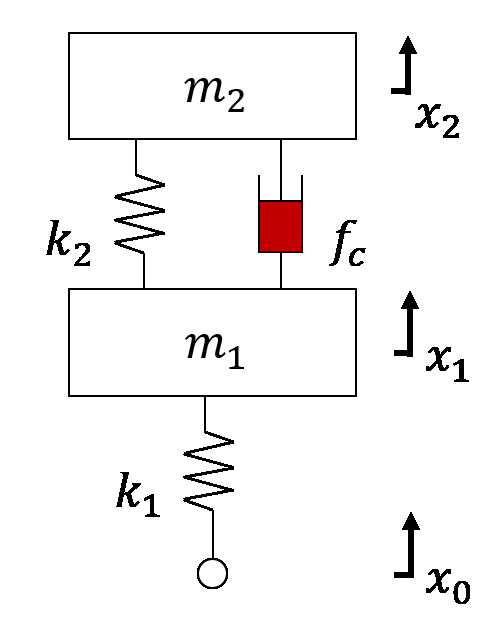
\includegraphics[height=30mm]{figure/analysis_model.eps}
      \vspace*{1mm}
      \caption{Analysis Model}
    \label{fig:analysis_model}
    \end{center}
  \end{minipage}
  \begin{minipage}{0.35\hsize}
      \begin{center}
	\makeatletter
	\def\@captype{table}
	\makeatother
	\caption{Parameter}
	\label{tab:parameter}
	  \begin{tabular}{cc}\hline
	    $m_1$ [kg] & 1.3\\
	    $m_2$ [kg] & 6.9\\
	    $k_1$ [N/m] & 2200\\
	    $k_2$ [N/m] & 439\\\hline
	  \end{tabular}
      \end{center}
  \end{minipage}
\end{figure}

\subsection{試験機}
本研究で使用するHILS試験機を図\ref{eq:2dof_m1}に示す.この装置は上下1自由度で


\section{IDCS制御手法}

\section{HILS試験}

\begin{thebibliography}{99}
\bibitem{hils}永井正夫,吉田秀久,Noomwongs Nuksit,横井隆,川眞田智,小林克宏,タイヤHILシミュレータによる車両運動性のの研究(第1報):タイヤHILシミュレータの開発,自動車記述会論文集,Vol.35,No.2,(2004),pp.147-152
\bibitem{2dof}社団法人 自動車技術会,自動車技術ハンドブック5設計(シャシ)編,社団法人 自動車技術会,(1990),p.25
\end{thebibliography}

\end{document}
